\documentclass[a4paper, 12pt, oneside]{book}

\usepackage[utf8]{inputenc}
\usepackage{lmodern}
\usepackage{layout}
\usepackage{emptypage}
\usepackage{fancyhdr}
\usepackage{subfigure} % subfiguras
\usepackage{caption}
\usepackage{mathtools}
\usepackage{hyperref}
\usepackage[a4paper,top=3cm, bottom=3cm, inner=2.5cm, outer=2.5cm]{geometry}
\usepackage{listings}
\usepackage[spanish]{babel}
\usepackage{url}
\usepackage{float}
\usepackage{multirow}
\usepackage{rotating} 
\usepackage{color}
\usepackage{colortbl}
\usepackage[table]{xcolor}
\usepackage[spanish]{babel}
\usepackage{tikz}
\usetikzlibrary{shapes.geometric, arrows}
\usepackage[bottom]{footmisc}
\usepackage{amssymb}



\tikzset{
  treenode/.style = {shape=rectangle, rounded corners,
                     draw, anchor=center,
                     text width=3cm, align=center,
                     top color=white, bottom color=blue!20,
                     inner sep=1ex},
  treenodelong/.style = {shape=rectangle, rounded corners,
                     draw, anchor=center, minimum height = 1cm,
                     text width=6cm, align=center,
                     top color=white, bottom color=blue!20,
                     inner sep=1ex},
  decision/.style = {treenode, diamond,  aspect=2, inner sep=0pt,
                     text centered, draw=black},
  arrow/.style = {thick,->,>=stealth}
}

\usepackage{dirtree}
\usepackage{mdwlist}


\usepackage[acronym, nonumberlist]{glossaries}
\makeglossaries
\newacronym{urm}{MRU}{Movimiento Rectilíneo Uniforme}
\newacronym{dof}{DOF}{Grado de libertad}
\newacronym{dofs}{DOF}{Grados de libertad}
\newacronym{mlp}{MLP}{\textit{Multilayer Perceptron}}
\newacronym{lstm}{LSTM}{\textit{Long Short-Term Memory}}

\makeatletter
\renewcommand{\@makeschapterhead}[1]{%
%  \vspace*{50\p@}%
  \vspace*{0\p@}%
  {\parindent \z@ \raggedright
    \normalfont
    \interlinepenalty\@M
    \Huge \bfseries  #1\par \nobreak
%    \vskip 40\p@
    \vskip 15\p@
  }}
\makeatother

\renewcommand{\baselinestretch}{1.4}
\setlength{\headheight}{16pt} 
\captionsetup{justification=justified}
\pretolerance=1000

\chead[]{}
\rhead[]{}
\renewcommand{\headrulewidth}{0.5pt}

\pagestyle{empty}

\title{Predicción de fotogramas}
\author{Nuria Oyaga de Frutos}

\lstset{
	float=hbp,
	basicstyle=\ttfamily\small,
	columns=flexible,
	tabsize=4,
	frame=single,
	extendedchars=true,
	showspaces=false,
	showstringspaces=false,
	numbers=none,
	numberstyle=\tiny,
	breaklines=false,
	breakautoindent=true,
	captionpos=b
}
\setcounter{tocdepth}{4}
\setcounter{secnumdepth}{4}

\definecolor{lightgray}{gray}{0.9}

\begin{document}
%%%%%%%%%%%%%%% Portada %%%%%%%%%%%%%%%%%%%%
\begin{titlepage}
	\begin{center}
		\begin{center}
			
\includegraphics[width=0.4\linewidth]{figures/logo}
		\end{center}
		\vspace{7.5mm}
		
		\fontsize{15.5}{14}\selectfont ESCUELA TÉCNICA SUPERIOR DE INGENIERÍA INFORMÁTICA
		\vspace{13mm}
		
		\fontsize{14}{14}\selectfont MÁSTER UNIVERSITARIO EN VISIÓN ARTIFICIAL 
		
		\vspace{70pt}
		
		\fontfamily{lmss}\fontsize{15.7}{14}\selectfont \textbf{TRABAJO FIN DE MÁSTER} 
		
		\vspace{20mm}
		\begin{huge}
			Predicción de fotogramas \vspace{0.4cm} \\ con Redes Neuronales
		\end{huge}
		
		\vspace{35mm}
		
		\begin{large}
			Autor: Nuria Oyaga de Frutos
			
			Tutor: José María Cañas Plaza
			
			Cotutor: Inmaculada Mora Jiménez
			
			\vspace{20mm}
		\end{large}
		\begin{normalsize}
			Curso académico 2019/2020	
		\end{normalsize}
		\vspace{10mm}
		
	\end{center}
	
\end{titlepage}

\pagebreak
\thispagestyle{empty}
\vspace*{12cm}

\begin{flushright}


\includegraphics[height=1.0cm]{figures/CC-BY-SA.png}

\vspace*{0.5cm}

\copyright 2020 Nuria Oyaga de Frutos

\vspace*{0.3cm}

Esta obra está distribuida bajo la licencia de 

``Reconocimiento-CompartirIgual 4.0 Internacional (CC BY-SA 4.0)''

de Creative Commons.

\vspace{0.2cm}

Para ver una copia de esta licencia, visite

http://creativecommons.org/licenses/by-sa/4.0/ o envíe

una carta a Creative Commons, 171 Second Street, Suite 300,

San Francisco, California 94105, USA.

\end{flushright}

\pagenumbering{Roman}

%%%%%%%%%%%%%%% Agradecimientos %%%%%%%%%%%%
{
	\vspace*{1cm}
	\begin{flushright}
		\textit{"The way to get started is to quit talking and begin doing"}\\
		\vspace{10pt}
		-Walt Disney-
	\end{flushright}
	
	\vspace*{14cm}
	\begin{flushright}
		\textit{A mi rosa mas bonita,\\
		la más bella del rosal,\\
		gracias por enseñarme,\\
		lo que es vivir y luchar.}
	\end{flushright}
}

\chapter*{Agradecimientos}

En primer lugar quiero dar las gracias...\\

\begin{flushright}
	\emph{¡Muchísimas gracias a todos!}
\end{flushright}


%%%%%%%%%%%%%%% Resumen %%%%%%%%%%%%%%%%%%%%
\chapter*{Resumen}

En los últimos años, la investigación en Visión Artificial para que las máquinas puedan percibir el mundo físico que les rodea, al igual que hace el ser humano mediante la vista, ha experimentado un gran desarrollo. En este aspecto, el uso de arquitecturas neuronales profundas cuyo aprendizaje está dirigido por conjuntos de datos representativos de la tarea a abordar, ha permitido mejorar las prestaciones de los algoritmos tradicionales. De las tres tareas que pueden realizar las estructuras neuronales, detección, clasificación y predicción, la predicción visual es la menos común. Además, dicha tarea tiene un largo recorrido en su investigación y una gran utilidad. Es por ello que este trabajo fin de máster aborda la tarea de predicción haciendo uso de secuencias de imágenes con un elemento móvil.\\

Se ha realizado un estudio sobre cómo distintas estructuras neuronales, de naturaleza recurrente y no recurrente, pueden utilizarse para realizar la predicción de fotogramas en una secuencia de vídeo, donde las correlaciones espacio-temporales entre imágenes son importantes. Para ello, se ha creado una serie de secuencias sintéticas formadas por fotogramas en los que un único píxel activo se desplaza siguiendo una determinada dinámica temporal: lineal, parabólica o sinusoidal. Así mismo, se han considerado los fotogramas en dos formatos distintos, uno modelado, que reduce toda la imagen a las posiciones (\textit{x}, \textit{y}) del píxel activo, y otro crudo, que representa la imagen como una matriz 2D de píxeles. Para obtener las secuencias sintéticas,  se ha desarrollado un generador que permite crear ejemplos adaptados a un tipo de estudio concreto.\\

Con la realización de esta investigación se ha comprobado que, bajo determinadas hipótesis, es posible predecir satisfactoriamente la posición del objeto móvil en secuencias de imágenes. Además, la recurrencia en las estructuras neuronales aporta un gran valor para abordar este tipo de tarea, pues permite capturar la correlación temporal existentes en la secuencia.


%%%%%%%%%%%%%%% Índices %%%%%%%%%%%%%%%%%%%%
\renewcommand{\tablename}{Tabla}
\renewcommand{\listtablename}{Índice de tablas}
\tableofcontents

\cleardoublepage % Í­ndice de figuras
\addcontentsline{toc}{chapter}{\listfigurename}
\listoffigures

\cleardoublepage % Í­ndice de tablas
\addcontentsline{toc}{chapter}{Índice de tablas}
\listoftables 


%%%%%%%%%%%%%%% Acronimos %%%%%%%%%%%%%%%%%%%%
\renewcommand{\acronymname}{Acrónimos}
\cleardoublepage
\addcontentsline{toc}{chapter}{Acrónimos}
\printglossary[type=\acronymtype]

\cleardoublepage
%%%%%%%%%%%%%%% Capítulos %%%%%%%%%%%%%%%%%%
\pagestyle{fancy}
\pagenumbering{arabic}
\setlength{\parindent}{6mm}

\lhead[]{CAPÍTULO \thechapter. INTRODUCCIÓN}
\chapter{Introducción}\label{cap.introduccion}
En este capítulo se situará el trabajo en el marco existente en la actualidad, explicando de manera genérica en qué consiste el aprendizaje profundo...

\section{Visión Artificial}

\section{Predicción}

\section{Redes neuronales artificiales}
\subsection{\acrfull{mlp}}
\subsection{Redes neuronales convolucionales}
\subsection{Redes neuronales recurrentes}
\subsubsection{Capas \acrfull{lstm}}
\subsubsection{Capas \textit{ConvLSTM}}
\lhead[]{CAPÍTULO \thechapter. OBJETIVOS}
\chapter{Objetivos}\label{cap.objetivos}
En este capítulo se expondrán los principales componentes software utilizados...

\section{Objetivos}

\section{Metodología}

\section{Plan de trabajo}

\lhead[]{CAPÍTULO \thechapter. ESTADO DEL ARTE}
\chapter{Estado del arte}\label{cap.estado}

\section{Predicción de valores}

\section{Predicción en imágenes}

\section{Infraestructura utilizada}
\subsection{Python}
\subsection{OpenCV}
\subsection{Keras}
\subsection{Tensorflow}
\subsection{Servidor Tamino}
\lhead[]{CAPÍTULO \thechapter. GENERACIÓN DE DATOS}
\chapter{Generación de datos}\label{cap.generacion}

En este capítulo se expondrá el código desarrollado para la generación de los conjuntos de datos que se emplean en los distintos experimentos de este trabajo. Así mismo, se explican los dos tipos de imágenes que se han considerado, modeladas y crudas, y se exponen las distintas dinámicas de movimiento entre \textit{frames} que se aplican dentro de un mismo conjunto.

\section{Propiedades del \textit{dataset}}

Esta sección hace hincapié en las características de los \textit{datasets} generados con secuencias de vídeo, objeto principal de estudio en este trabajo. Se explican en profundidad la estructura que tiene el directorio que almacena los distintos conjuntos utilizados, los dos tipos de imágenes considerados: modeladas y crudas, y las tres dinámicas que han sido estudiadas: lineal, parabólica y sinusoidal.

\subsection{Estructura del \textit{dataset}} \label{ap.estructura}

En la Figura~\ref{fig.estructura_dataset} se presenta un esquema de la estructura resultante con la ejecución del código explicado en la Sección~\ref{sec.generador} con diferentes parámetros (\textit{1..n})

\begin{figure}[H]
	\begin{center}
	    \setlength{\fboxsep}{0.5cm}
	    \fbox{
        \begin{minipage}{6.7cm}
          \dirtree{%
          .1 Frames dataset.
          .2 Specific parameters \textit{1}.
          .3 Train.
          .4 Modeled samples.
          .5 \textit{sample0.txt}.
          .5 \vdots.
          .4 Raw samples.
          .5 sample0.
          .6 \textit{0.png}.
          .6 \vdots.
          .5 \vdots.
          .4 \textit{parameters.txt}.
          .3 Test.
          .4 \vdots.
          .3 Val.
          .4 \vdots.
          .2 \vdots.
          .2 Specific parameters \textit{n}.
          }
        \end{minipage}
        }
	    \caption{Estructura del \textit{dataset}.}
	    \label{fig.estructura_dataset}
	\end{center}
\end{figure}
\vspace{-10pt}
En el primer nivel de esta estructura, \textit{Frames dataset}, se distinguen entre los distintos tipos de datos que se pueden generar. A pesar de que en este trabajo se ha centrado en las secuencias de imágenes, el generador fue diseñado para poder obtener otros dos tipos de datos: funciones y vectores, que tendrían su directorio homólogo en este mismo nivel.\\

En el segundo nivel se hace una distinción en función de los parámetros concretos que se hayan establecido en el fichero de configuración, explicado en el apartado~\ref{ap.fichero}. Estos valores son:

\begin{itemize}
    \setlength\itemsep{3pt}
    \item Tipo de dinámica.
    \item Forma y color del objeto.
    \item Grados de libertad.
    \item Número de muestras.
    \item Tamaño de la imagen.
\end{itemize}

A pesar de que existen otros valores diferenciales, como el número de elementos conocidos, en este trabajo no han sido modificados, por lo que no se incluyen en el nombre del directorio. El \textit{gap} con el elemento a predecir es especificado en el siguiente nivel.\\

Dentro de cada uno de estos directorios se presenta siempre la misma estructura. La primera división existente es la de los subconjuntos de entrenamiento, \textit{test} y validación. Si no se hubiese indicado la realización de esta división, este nivel sería obviado y se pasaría directamente al siguiente. Todas estas carpetas presentan a su vez la misma estructura, sobre la que la herramienta de generación escribe directamente las distintas muestras: el fichero de parámetros, la carpeta con las muestras modeladas y la correspondiente a las muestras en crudo. En el apartado~\ref{ap.tip_img} se explica de forma más concreta en qué consiste cada una de estas muestras.

\subsection{Tipos de imágenes} \label{ap.tip_img}

Se han considerado dos tipos de imágenes para los distintos estudios que se han desarrollado en el trabajo. Ambos tipos de imágenes tienen una correspondencia entre sí, es decir, para una misma muestra se presenta la misma información en dos formatos distintos: valores numéricos e imágenes.

\subsubsection{Imágenes modeladas}

Las datos modelados son una forma simplificada de mostrar las distintas posiciones que adquiere el píxel en cada instante de tiempo. En la Tabla~\ref{tab.modelada} se presenta un ejemplo concreto de cómo se representan estas muestras.

\begin{table}[H]
	\centering
	\begin{tabular}{{l|c|c|}}
		\hline
		\multicolumn{1}{|l|}{\textbf{\textit{t}}} & \textbf{\textit{x}} & \textbf{\textit{y}}\\\hline 
		\multicolumn{1}{|l|}{\textbf{0}} & 0 & 40\\ \hline
		\multicolumn{1}{|l|}{\textbf{1}} & 3 & 38\\ \hline
		\multicolumn{1}{|l|}{\textbf{2}} & 6 & 37\\ \hline
		\multicolumn{1}{|l|}{\textbf{3}} & 9 & 36\\ \hline
		\multicolumn{1}{|l|}{\textbf{\vdots}} & \vdots & \vdots\\ \hline
		\multicolumn{1}{|l|}{\textbf{29}} & 87 & 4\\ \hline
		
	\end{tabular}
	\caption{Ejemplo de muestra modelada.}
	\label{tab.modelada}
\end{table}

Estos datos se almacenan en la carpeta \textit{modeled}\_\textit{samples} mediante un fichero \textit{"sample[n].txt}, donde \textit{n} hace referencia al número del ejemplo durante su creación. Este fichero presenta una cabecera y un número de filas que se corresponde al número de instantes conocidos más el instante que se quiere predecir. La información viene distribuida en dos columnas, correspondientes con los valores \textit{x} e \textit{y} del píxel en cada instante de tiempo, que no se representa de forma explícita sino que se asocia con el orden de las filas.\\

Con este tipo de imágenes se consigue representar la misma información de una forma más compacta, se utiliza un total de \textit{$2 * n\_points$}  valores de entrada a la red, y \textit{$2$} valores de salida de la misma, reduciendo considerablemente la complejidad de las distintas redes que se estudien.

\subsubsection{Imágenes crudas}

Las imágenes crudas son las imágenes propiamente dichas. En la Figura~\ref{fig.cruda} se muestra una composición con todas las imágenes que forman la secuencia agrupadas en una única imagen.

\begin{figure}[H]
		\begin{center}
			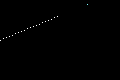
\includegraphics[width=0.6\textwidth]{Memoria-TFM/figures/samples/linear_sample.png}
			\caption{Ejemplo de muestra cruda.}
			\label{fig.cruda}
		\end{center}
\end{figure}
\vspace{-10pt}
Cada uno de las fotogramas presentaría un único píxel activo que se corresponde con el objeto del que se simula el movimiento y se almacena con el nombre \textit{"[n].png"} en la carpeta \textit{"sample[m]"}, donde \textit{"n"} sería el orden del instante de tiempo y \textit{"m"} el de la muestra generada. Cada una de estas carpetas que identifica una muestra es almacenada en el directorio \textit{raw}\_\textit{samples} que confluye todos los ejemplos del mismo tipo.\\

En este caso, a pesar de que la información es la misma, la cantidad de valores que se utilizan para representarla es mucho mayor. Se utiliza un total de \textit{$h * w * n\_points$}  valores de entrada a la red, y \textit{$h * w$} valores de salida de la misma, complicando las redes a estudiar.

\subsection{Tipos de dinámicas} \label{ap.dinamicas}

El movimiento del píxel en el vídeo viene determinado por tres dinámicas distintas, que van aumentando el grado de complejidad del mismo y ponen a prueba la capacidad de predicción de las redes. Además de las tres dinámicas que se han considerado: lineal, parabólica y  sinusoidal, dentro de cada una de ellas se aumenta de forma escalonada la dificultad incrementando el número de variables que adquieren un valor aleatorio, es decir, los \acrfull{dof} de las mismas.\\

Como se explica en el apartado~\ref{ap.generacion}, estas dinámicas afectan únicamente a la posición \textit{y} del píxel, y se utilizan los valores de \textit{x} obtenidos mediante la aplicación de un \acrfull{urm} al instante de tiempo con una velocidad aleatoria.\\

\subsubsection{Dinámica lineal}

La primera dinámica, y la más sencilla de todas, simula el movimiento del objeto en una línea recta a distintas velocidades y con distintas pendientes. Este movimiento se puede asimilar con el movimiento de un vehículo con una velocidad constante, sin tener en cuenta los efectos del rozamiento por la superficie. Para ello, utiliza la ecuación de la recta:
$$y = m*x + y0$$
que se materializa en el código de la siguiente forma:
\vspace{10pt}
\begin{lstlisting}[frame=single]
  self.g = lambda x, y0, m: (m * x) + y0
\end{lstlisting}

En la Figura~\ref{fig.lineal} se presenta un ejemplo de esta dinámica con todas las imágenes que lo conforman superpuestas en una sola.

\begin{figure}[H]
		\begin{center}
			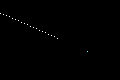
\includegraphics[width=0.6\textwidth]{Memoria-TFM/figures/samples/linear2_sample.png}
			\caption{Ejemplo de dinámica lineal.}
			\label{fig.lineal}
		\end{center}
\end{figure}

Por la propia naturaleza de la ecuación, es posible ir modificando la complejidad del movimiento a medida que incrementamos la cantidad de parámetros que se asignan de forma aleatoria, es decir, los \acrshort{dof}. A continuación, se exponen los distintos casos que se dan en la dinámica actual.

\begin{description}
\item[\textbf{Movimiento \acrshort{urm}}] \hfill 
\vspace{10pt}
\\
El movimiento más sencilla que se puede encontrar es un caso especial de la dinámica lineal. Ocurre cuando todos se fija la pendiente de la recta (\textit{m}) en un valor nulo, igualando el valor de la posición a una altura inicial. De esta forma se obtiene la ecuación simplificada:
$$y = y0$$
que se presenta en el código de la siguiente manera:
\vspace{10pt}
\begin{lstlisting}[frame=single]
  self.g = lambda x, y0: y0
\end{lstlisting}
La altura inicial se puede asignar de dos maneras distintas::
\vspace{10pt}
\begin{lstlisting}[frame=single]
  y0 = int(self.h / 2) #1
  y0 = random.randint(1, self.h - 1) #2
\end{lstlisting}
La primera línea asigna la altura a la mitad de la imagen (\textit{h/2}), mientras que con la segunda se establece un valor aleatorio entre los límites de la imagen, que introduce un nuevo \acrshort{dof}.

En la Figura~\ref{fig.urm} se muestra un ejemplo de este caso especial de la dinámica lineal.

\begin{figure}[H]
		\begin{center}
			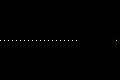
\includegraphics[width=0.6\textwidth]{Memoria-TFM/figures/samples/URM_sample.png}
			\caption{Ejemplo del caso \acrshort{urm}}
			\label{fig.urm}
		\end{center}
\end{figure}
\vspace{-10pt}

\item[\textbf{1 \acrshort{dof}}] \hfill 
\vspace{10pt}
\\
El primer parámetro de la ecuación que toma un valor aleatorio en cada muestra es la pendiente de la recta, dejando fija la altura inicial del punto. El código que se utiliza en cada iteración para la definición de los parámetros es el siguiente:
\vspace{10pt}
\begin{lstlisting}[frame=single]
  m = np.round(random.uniform(-self.h/10, self.h/10), 2)
  y0 = int(self.h / 2)
\end{lstlisting}
Los límites que se establecen para obtener el valor aleatorio son orientativos. Pretenden reducir al máximo el intervalo que asegure la presencia del punto en todas las imágenes pero esta presencia no llega a asegurarse en su totalidad. Es por esto que, posteriormente, se realiza una comprobación de las posiciones obtenidas.
\vspace{10pt}
	
\item[\textbf{2 \acrshort{dof}}] \hfill 
\vspace{10pt}
\\
Se deja que todos los parámetros de la ecuación tomen un valor aleatorio distinto en cada muestra, tanto la pendiente como la altura inicial. Para esta asignación se implementa el siguiente código:
\vspace{10pt}
\begin{lstlisting}[frame=single]
  m = np.round(random.uniform(-self.h/10, self.h/10), 2)
  y0 = random.randint(1, self.h - 1)
\end{lstlisting}
Al igual que en el caso anterior, los límites establecidos son orientativos para cumplir con las limitaciones del \textit{dataset}.
\vspace{10pt}

\end{description}

\subsubsection{Dinámica parabólica}

La dinámica parabólica, que aumenta el grado de complejidad mediante el incremento del número de parámetros necesarios para su definición, utiliza la ecuación de la parábola para obtener las posiciones \textit{y}:
$$y = a*t^2 + b*t + c$$
que se implementa en el código de mediante las siguiente línea:
\vspace{10pt}
\begin{lstlisting}[frame=single]
  self.g = lambda x, a, b, c: a * (x ** 2) + b * x + c
\end{lstlisting}

En la Figura~\ref{fig.parab} se puede ver un ejemplo, con el mismo formato que el de la dinámica anterior, de este tipo de movimiento.

\begin{figure}[H]
		\begin{center}
			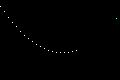
\includegraphics[width=0.6\textwidth]{Memoria-TFM/figures/samples/parabolic_sample.png}
			\caption{Ejemplo de dinámica parabólica.}
			\label{fig.parab}
		\end{center}
\end{figure}
\vspace{-10pt}

Al igual que en el caso lineal, se va incrementando la complejidad de la dinámica  aumentando el número de \acrshort{dof}, explicados a continuación.

\begin{description}
\item[\textbf{1 \acrshort{dof}}] \hfill 
\vspace{10pt}
\\
El parámetro que se modifica en este primer caso es el que acompaña al término cuadrático (\textit{a}), de tal forma que la definición de los parámetros queda de la siguiente manera: 
\vspace{10pt}
\begin{lstlisting}[frame=single]
  a = round(random.uniform(-0.75, 0.75), 3)
  b = 1.5
  c = int(self.h / 2)
\end{lstlisting}
El valor otorgado a \textit{b} deriva de una serie de pruebas para obtener aquel que mejor se ajustase a lo que se buscaba mientras que la altura inicial (\textit{c}) se establece en la mitad de la imagen. Por otro lado, al igual que ocurre en la dinámica lineal, los límites escogidos son orientativos para cumplir con la presencia del píxel en todas las imágenes, pero en ningún caso la asegura. 
\vspace{10pt}
	
\item[\textbf{2 \acrshort{dof}}] \hfill 
\vspace{10pt}
\\
El siguiente parámetro a modificar es el homólogo al de la dinámica lineal: la altura inicial, que en este caso se establece con el parámetro \textit{c}. Siguiendo la definición del caso lineal,los parámetros de este caso quedan definidos de la siguiente manera:
\vspace{10pt}
\begin{lstlisting}[frame=single]
  a = round(random.uniform(-0.75, 0.75), 3)
  b = 1.5
  c = random.randint(1, self.h - 1)
\end{lstlisting}
Al igual que en el caso anterior, los límites establecidos son orientativos para cumplir con las limitaciones del \textit{dataset}.
\vspace{10pt}

\item[\textbf{3 \acrshort{dof}}] \hfill 
\vspace{10pt}
\\
El último caso se definen todos los parámetros de la ecuación mediante un valor aleatorio. Con esta premisa, la definición de los parámetros presenta la siguiente forma:
\vspace{10pt}
\begin{lstlisting}[frame=single]
  a = round(random.uniform(-0.75, 0.75), 3)
  b = round(random.uniform(-2, 2), 3)
  c = random.randint(1, self.h - 1)
\end{lstlisting}
\vspace{10pt}

\end{description}

\subsubsection{Dinámica sinusoidal}
La dinámica más compleja considerada en este trabajo, la sinusoidal, hace uso de la función trigonométrica del seno para el cálculo de posiciones en el eje vertical. Su expresión es la siguiente:
$$y = a*sin(2*\pi*f*x + b) + c$$
y se traduce en el código en la línea:
\vspace{10pt}
\begin{lstlisting}[frame=single]
  self.g = lambda x, a, b, c, f: 
    a * math.sin(2 * math.pi * f * math.radians(x) + b) + c
\end{lstlisting}

En la Figura~\ref{fig.sin} se muestra un ejemplo de la dinámica mediante la superposición de las imágenes en una sola.

\begin{figure}[H]
		\begin{center}
			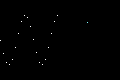
\includegraphics[width=0.6\textwidth]{Memoria-TFM/figures/samples/sinusoidal_sample.png}
			\caption{Ejemplo de dinámica sinusoidal.}
			\label{fig.sin}
		\end{center}
\end{figure}

De la misma forma que sucede con las otras dos dinámicas, se aumenta la dificultad del movimiento mediante el aumento  de los \acrshort{dof}, que se exponen a continuación.\\

\begin{description}
\item[\textbf{1 \acrshort{dof}}] \hfill 
\vspace{10pt}
\\
El primer parámetro que se establece de forma aleatoria es la frecuencia (\textit{f}) del seno. La definición de los parámetros para este caso queda de la siguiente manera:\\
\vspace{10pt}
\begin{lstlisting}[frame=single]
  a = 25
  f = round(random.uniform(0.5, 5), 2)
  b = 0
  c = int(self.h / 2)
\end{lstlisting}

Como ocurre en el caso parabólico, los valores de los parámetros fijados se han obtenido mediante distintas pruebas con el objetivo de que sean lo más adecuados para los estudios realizados. De igual forma, los límites establecidos son orientativos para cumplir con las limitaciones del \textit{dataset}.
\vspace{10pt}
	
\item[\textbf{2 \acrshort{dof}}] \hfill
\vspace{10pt}
\\
El segundo parámetro que se deja libre es, de nuevo, el homólogo a los casos anteriores. Se trata de la altura inicial de la imagen en la que comienza el movimiento, dando lugar a la siguiente definición de parámetros:
\vspace{10pt}
\begin{lstlisting}[frame=single]
  a = 25
  f = round(random.uniform(0.5, 5), 2)
  b = 0
  c = random.randint(1, self.h - 1)
\end{lstlisting}
Al igual que en el caso anterior, 
\vspace{10pt}

\item[\textbf{3 \acrshort{dof}}] \hfill 
\vspace{10pt}
\\
El tercer parámetro que obtiene valores aleatorios en esta dinámica es la amplitud del seno, y se definen los parámetros de este caso con el siguiente código:
\vspace{10pt}
\begin{lstlisting}[frame=single]
  a = random.randint(15, 40)
  f = round(random.uniform(0.5, 5), 2)
  b = 0
  c = random.randint(1, self.h - 1)
\end{lstlisting}
\vspace{50pt}

\item[\textbf{4 \acrshort{dof}}] \hfill 
\vspace{10pt}
\\
Por último, al igual que en la dinámica lineal y la parabólica, se permite que todos los parámetros tomen valores aleatorios, dando lugar al caso más complejo de este movimiento. El código utilizado para definir los parámetros en este último caso es:
\vspace{10pt}
\begin{lstlisting}[frame=single]
  a = random.randint(15, 40)
  f = round(random.uniform(0.5, 5), 2)
  b = round(random.uniform(0, 2 * math.pi), 3)
  c = random.randint(1, self.h - 1)
\end{lstlisting}
\vspace{10pt}
\end{description}

\section{Herramienta de generación} \label{sec.generador}

Para la elaboración propia de los distintos conjuntos de datos,  se ha desarrollado un código en Python que, a través de la fijación de varios parámetros, elabora un conjunto de muestras que se adapta al estudio concreto en el que se vaya a aplicar. En esta sección se explican las dos partes fundamentales de este código: la especificación de los parámetros y la propia generación y almacenamiento de las muestras.

\subsection{Fichero de configuración} \label{ap.fichero}

A través de este fichero se establecen los parámetros principales que definen las características del \textit{dataset} a generar. A continuación se explican los distintos valores a definir y lo que supone modificar cada uno de ellos. 

\begin{basedescript}{\desclabelstyle{\pushlabel}\desclabelwidth{2.75cm}}
\item[\textit{root}] Define la ruta en la que se almacenará la estructura de carpetas y archivos que se genera en la ejecución del código.
\item[\textit{to\_generate}] Indica el tipo de dato que va a ser generado. A pesar de que este proyecto se centra en el estudio con imágenes, el generador se desarrolló con la posibilidad de generar datos de tres tipos: funciones, vectores unidimensionales e imágenes.
\item[\textit{motion\_type}] Especifica el tipo de movimiento que sigue el objeto entre cada \textit{frame}, explicadas en el apartado~\ref{ap.dinamicas}.
\item[\textit{height}]  Número entero que indica la altura de la imagen, su dimensión \textit{y}.
\item[\textit{width}]  Número entero que indica el ancho de la imagen, su dimensión \textit{x}.
\item[\textit{object}]  Define el tipo de objeto que se mueve en la imagen. En este trabajo únicamente se utiliza el objeto píxel, de tal forma que toda la imagen será negra a excepción de un punto activo que será considerado el objeto.
\item[\textit{obj\_color}]  Permite definir el color del objeto. Se utiliza un único nivel de intensidad en el caso del píxel y una terna RGB para otros objetos.
\item[\textit{dof}] Establece los grados de libertad de la dinámica de movimiento, es decir, el número de variables que se generan de forma aleatoria en la ecuación que la define.
\item[\textit{n\_samples}]  Número entero que indica el número de muestras totales que se generarán en el conjunto.
\item[\textit{n\_points}] Número entero que indica la cantidad de instantes de tiempo que serán utilizados para predecir.
\item[\textit{gap}] Número entero que define la separación temporal, instantes de tiempo, entre la última muestra conocida y la muestra a predecir.
\item[\textit{noise}] Permite añadir ruido de un determinado tipo a las muestras para un estudio más avanzado.
\item[\textit{split}] Indica si se dividirá el conjunto en los tres subconjuntos y la proporción en la que lo hará si así de define.
\end{basedescript}

De esta manera, se permite un ajuste más sencillo del \textit{dataset} a generar al tipo de problema que se quiera estudiar, dejando al gusto del usuario las características del mismo.
    
\subsection{Generación del \textit{dataset}} \label{ap.generacion}

En la Figura~\ref{fig.flujo_gen} se expone el diagrama del flujo que sigue el programa encargado de la generación del \textit{dataset}, centrándose en el tipo de dato que es es de interés en este trabajo: los fotogramas.\\
\vspace{10pt}
\begin{figure}[H]
    \begin{center}
        \begin{tikzpicture}[node distance=2.5cm]
            \node (cd) [treenode] {Creación de \\ directorios};
            \node (def) [treenode, below of=cd] {Definición de muestra};
            \node (obt) [treenode, below of=def] {Obtención de muestra};
            \node (val) [decision, below of=obt, yshift=-0.25cm] {¿Es válida?};
            \node (gen) [treenode, below of=val, yshift=-0.25cm] {Generación de imágenes};
            \node (div) [decision, below of=gen, yshift=-0.25cm] {¿División?};
            \node (asig) [treenode, below of=div, yshift=-0.25cm] {Asignación de subconjunto};
            \node (sav) [treenode, right of=div, xshift=3cm] {Almacenamiento de muestras};
            
            \draw [arrow] (cd) -- (def);
            \draw [arrow] (def) -- (obt);
            \draw [arrow] (obt) -- (val);
            \draw [arrow] (val) -- node[anchor=east, yshift=0.3cm] {Sí} (gen);
            \draw [arrow] (val) --  node[anchor=south, xshift=-0.35cm] {No} ++ (3cm,0cm) |-(obt);
            \draw [arrow] (gen) -- (div);
            \draw [arrow] (div) -- node[anchor=east, yshift=0.3cm] {Sí} (asig);
            \draw [arrow] (div) --  node[anchor=south, xshift=-0.6cm] {No} (sav);
            \draw [arrow] (asig) -- ++ (5.5cm,0cm) |- (sav.south);
            \draw [arrow] (sav) |- node[align=center, anchor=west, yshift=-5cm, xshift=0.2cm] {\textit{for n in}\\ \textit{n}\_\textit{samples}} (def);
        \end{tikzpicture}
        \caption{Diagrama de flujo del generador.}
	    \label{fig.flujo_gen}
	\end{center}
\end{figure}
\vspace{-10pt}
En primer lugar se comprueban y se crean, en caso de ser necesario, los directorios que son necesarios para el almacenamiento del conjunto según la ruta que ha sido indicada en el fichero de configuración. La estructura de ficheros que se crea con el fin de almacenar todas las muestras del conjunto es explicada en el apartado~\ref{ap.estructura}.\\
\vspace{20pt}
\\
Tras la creación de la estructura necesaria se entra en un bucle, que se itera el número de muestras que haya sido definido, en el que se define, obtiene, valida, genera y almacena cada uno de los ejemplos que conforman el \textit{dataset}.\\

Para la definición de la muestra se utiliza la clase correspondiente al tipo de movimiento que se vaya a implementar, la cual tiene definida de forma interna la ecuación que se corresponde con la dinámica. Este tipo de dinámica a implementar viene indicada en el fichero de configuración, como se explicó anteriormente, y todas las clases y ecuaciones que son utilizadas se explican en profundidad en el apartado
~\ref{ap.dinamicas}.\\

Tras definir la muestra se llama a la función encargada de generarla. A grandes rasgos, esta función obtiene las posiciones \textit{(x,y)} del píxel en cada uno de los \textit{frames} y comprueba que esta posición obtenida no se salga de los límites de la imagen, evitando así oclusiones y desapariciones. Para obtener esas posiciones se realizan varios pasos que, aunque pueden variar en número función de la dinámica y los grados de libertad, siguen siempre la misma estructura. Esta estructura queda encapsulada en un bucle \textit{while}, que será detenido una vez se obtenga un conjunto de posiciones válidas, con las siguientes operaciones:

\begin{enumerate}
  \item Se define el movimiento que sigue el píxel en el eje \textit{x}, identificado con el instante temporal \textit{t} y, por tanto, con la velocidad a la que se mueve el píxel. Éste es el mismo independientemente de la dinámica con la que se esté trabajando, se corresponde con un \acrshort{urm} y viene definido de la siguiente forma:
  \vspace{10pt}
  \begin{lstlisting}[frame=single]
  self.f = lambda t, x0, u_x: x0 + u_x * t
  \end{lstlisting}
  Para poder definir el movimiento \acrshort{urm} en los conjuntos desarrollados se fija el punto de inicio (\textit{x0}) en el instante 0 y se asigna una velocidad aleatoria para cada una de las muestras. Esta asignación se realiza mediante el siguiente código:
  \vspace{10pt}
  \begin{lstlisting}[frame=single]
  limit = int(self.w / (self.n_points + self.gap))
  u_x = random.randint(1, limit)
  \end{lstlisting}
  Así se establece un límite en la velocidad, en función del número de instantes de tiempo conocidos y la separación entre el instante a predecir y el último conocido, que asegura la aparición del píxel en todas las imágenes.
  
  \item Se obtienen los valores concretos de la posición \textit{x} en cada instante de tiempo de la siguiente forma:
  \vspace{10pt}
  \begin{lstlisting}[frame=single]
  numbers_x = [self.f(x, x0, u_x) for x in range(self.n_points)]
  numbers_x.append(self.f(self.n_points + self.gap - 1, x0, u_x))
  \end{lstlisting}
  Primero se calculan todos los valores de los instantes de tiempo conocidos (\textit{n}\_\textit{points}) y, posteriormente, se añade el valor correspondiente con el instante a predecir (\textit{n}\_\textit{points+gap}).
  
  \item Se define el valor de todas las variables que son necesarias para aplicar la ecuación de la dinámica y obtener las posiciones en el eje \textit{y}. La forma de definir estas variables, explicadas en el el apartado~\ref{ap.dinamicas}, dependen del grado de libertad que se haya indicado en el fichero de configuración. A medida que aumenta la complejidad aumenta el número de variables que se generan de forma aleatoria. 
  
  \item Se calculan las posiciones en el eje \textit{y}, en función de la dinámica que se haya establecido, mediante la siguiente línea:
  \vspace{10pt}
  \begin{lstlisting}[frame=single]
  numbers_y = [self.g(n_x, *args) for n_x in numbers_x]
  \end{lstlisting}
  Los argumentos que se pasan a la función de la dinámica serán las variables que previamente han sido definidas.
  
  \item Se comprueba que todos las posiciones se encuentren dentro de la imagen y, en caso positivo, se detiene el bucle y se continúa con el flujo del programa de generación. Si es negativo se repetirá el proceso hasta alcanzar un conjunto de posiciones válido.
\end{enumerate}

Una vez se han obtenido las posiciones del píxel válidas se procede a la generación de la propia secuencia de imágenes. Para ello se recorren todas las posiciones que han sido generadas (\textit{n}\_\textit{points} + 1) y se crea una imagen por cada una de ellas. La imagen se inicia con todos los píxeles nulos, completamente negra, y posteriormente se activa el píxel que se corresponde con la posición \textit{(y,x)} con el valor indicado en el fichero de configuración, para este proyecto fijado en 255. Se debe trasponer el vector de posición por la forma en la que Numpy establece el acceso a las posiciones en las imágenes\footnote{\url{https://scikit-image.org/docs/dev/user\_guide/numpy_images.html}}, primero las filas (\textit{y}) y luego a las columnas (\textit{x}).

Antes de almacenar la muestra, si se ha establecido la división del \textit{dataset} en los subconjuntos de entrenamiento, validación y \textit{test}, se asignará la misma al conjunto al que pertenece. Para esta asignación se utiliza un criterio de orden de la siguiente forma:

\begin{itemize}
    \setlength\itemsep{3pt}
    \item $n\_sample < n\_train \Rightarrow$ Conjunto de entrenamiento
    \item $n\_train \leqslant n\_sample < n\_train + n\_test\Rightarrow$ Conjunto de \textit{test}
    \item $n\_train + n\_test \leqslant n\_sample < n\_train + n\_test\ + n\_val \Rightarrow$ Conjunto de validación
\end{itemize}

Los valores que definen el número de muestras que tiene cada conjunto vienen dados por los distintos parámetros de división establecidos en el fichero de configuración. El código empleado para calcular estos valores es el siguiente:
\vspace{10pt}
\begin{lstlisting}[frame=single]
  n_test = int(n_samples * float(conf['split']['fraction_test']))
  n_val = int(n_samples * float(conf['split']['fraction_validation']))
  n_train = n_samples - n_val - n_test
\end{lstlisting}

Para el almacenamiento de la muestra en la carpeta correspondiente, la del subconjunto si se ha hecho división o la general en caso contrario, se realizan tres operaciones que permiten obtener información de la misma en distintos formatos.

\begin{itemize}
    \setlength\itemsep{3pt}
    \item \textbf{\textit{parameters.txt}}: Se escriben las distintas variables utilizadas para la generación de cada muestra. Cada fila de este fichero se corresponde con un ejemplo generado.
    \item \textbf{\textit{modeled}\_\textit{samples}}: Se guarda un fichero para cada muestra con las posiciones de la misma.
    \item \textbf{\textit{raw}\_\textit{samples}}: Se almacena una carpeta por muestra con las imágenes que la conforman.
\end{itemize}

Con todo esto se obtiene un directorio, cuya estructura se explica más a fondo en el apartado~\ref{ap.estructura}, que contiene todo lo necesario para entrenar y evaluar las distintas redes que se estudian en el desarrollo de este proyecto.
\lhead[]{CAPÍTULO \thechapter. EVALUACIÓN Y MÉTRICAS}
\chapter{Evaluación y métricas}\label{cap.evaluacion}

En este capítulo se explican las distintas métricas que se calculan tras pasar el conjunto de \textit{test} por la red previamente entrenada, permitiendo obtener una medida objetiva de la bondad de dicha red. Además se hace un análisis en profundidad del código Python desarrollado para tal fin y se hace una interpretación sobre los gráficos y resultados que arroja dicho código al terminar la ejecución.

\section{Métricas}

Para poder evaluar la distin

\section{Herramienta de evaluación}

En la Figura~\ref{fig.flujo_test} se puede visualizar el flujo que sigue el código para la evaluación de una red en concreto con un conjunto de \textit{test} determinado.

\vspace{10pt}
\begin{figure}[H]
    \begin{center}
        \begin{tikzpicture}[node distance=2cm]
            \node (ld) [treenodelong] {Lectura de datos};
            \node (net) [treenodelong, below of=ld] {Carga de la red};
            \node (pred) [treenodelong, below of=net] {Predicción};
            \node (trans) [treenodelong, below of=pred] {Transformación de posiciones};    
            \node (calc) [treenodelong, below of=trans] {Cálculo de métricas};
            \node (pres) [treenodelong, below of=calc] {Presentación de resultados};
            
            \draw [arrow] (ld) -- (net);
            \draw [arrow] (net) -- (pred);
            \draw [arrow] (pred) -- (trans);
            \draw [arrow] (trans) -- (calc);
            \draw [arrow] (calc) -- (pres);
        \end{tikzpicture}
        \caption{Diagrama de flujo del evaluador.}
	    \label{fig.flujo_test}
	\end{center}
\end{figure}

\section{Interpretación de resultados}
\lhead[]{CAPÍTULO \thechapter. PREDICCIÓN DE IMÁGENES MODELADAS}
\chapter{Predicción de imágenes modeladas}\label{cap.redes3dmod}

En este capítulo se presentan todos los estudios realizados en cuanto a la predicción en imágenes modeladas, mejorando las redes en distintos factores según los resultados que se van obteniendo con el objetivo de encontrar la estructura más adecuada para predecir en el mundo real.\\

En el mundo de las imágenes modeladas se ha afrontado la predicción como un problema de regresión, en el que la entrada es el conjunto de instantes de tiempo que se consideran conocidos (\textit{n}\_\textit{points}) con sus pares de posiciones (\textit{x}, \textit{y}) y la salida es el instante de tiempo futuro con su par de coordenadas correspondiente. Cada uno de estas coordenadas pueden tomar cualquier valor numérico decimal por lo que, como se explicó en la Sección~\ref{sec.eval}, es necesario realizar un redondeo para obtener la posición final, pues los píxeles están siempre representados por números enteros.\\

A continuación se realiza el recorrido por las distintas estructuras entrenadas, presentando los resultados obtenidos y las conclusiones que dan lugar a la exploración de distintas vías para la mejora de los mismos.

\section{Redes no recurrentes}

\section{Redes recurrentes}
\subsection{Red básica}
\subsection{Aumento de neuronas}
\subsection{Aumento de capas}
\subsection{Red avanzada: Dinámica combinada}

\lhead[]{CAPÍTULO \thechapter. PREDICCIÓN DE IMÁGENES CRUDAS}
\chapter{Predicción de imágenes crudas}\label{cap.redes3dcrud}

\section{Redes no recurrentes}

\section{Redes recurrentes}
\subsection{Red básica}
\subsubsection{Convolución + LSTM VS \textit{ConvLSTM}}
\subsubsection{Estructura utilizada}
\subsection{Aumento de capas}
\subsection{Red avanzada: Dinámica combinada}

\lhead[]{CAPÍTULO \thechapter. CONCLUSIONES}
\chapter{Conclusiones}\label{cap.conclusiones}
En este capítulo se exponen las conclusiones alcanzadas con el desarrollo del proyecto, las aportaciones principales, así como posibles líneas para continuar el trabajo realizado.

\section{Conclusiones}

\section{Líneas futuras}



%%%%%%%%%%%%%%% Anexos %%%%%%%%%%%%%%%%%%%%%
%\lhead[]{CAPÍTULO \thechapter. ESTUDIOS PREVIOS}
%\include{7-Previos}
%%%%%%%%%%%%%%% Bibliografia %%%%%%%%%%%%%%%
\lhead[]{BIBLIOGRAFÍA}
\addcontentsline{toc}{chapter}{Bibliografía}
\bibliographystyle{unsrt}
\bibliography{Memoria}

\end{document}